Molecular modeling seeks to gain new insights into the real world behavior of molecules by mimicking these molecules, usually using computer simulations.
According to the theory of ``minimal frustration'' the protein native state is not only a low energy state, but is also stable \cite{bryngelson1987spin}.
So the prediction of native or native-like conformations focuses on finding those conformations which have a low potential energy.
As measuring the true potential energy of a system is very difficult or impossible computational models seek to reproduce the qualitative behavior of the energy surface.
Quantum mechanics calculations are often viewed as the gold standard with respect to intramolecular energy calculations.
However, despite the accuracy of quantum mechanics, its application to large systems such as proteins is currently limited due to the amount of time necessary to perform quantum mechanics calculations on a large number of atoms.
Instead quantum mechanics calculations have been used to parameterize a majority of the most popular molecular mechanics force fields currently in use, including:
\begin{enumerate}
\item AMBER \cite{weiner1984new},
\item OPLS-AA \cite{kaminski1994free},
\item and CHARMM \cite{mackerell2002charmm}.
\end{enumerate}

The earliest molecular mechanics force fields either modeled groups of atoms as a unit, hydrogens being grouped with their bound heavy atom \cite{jorgensen1988opls}, or even each residue as a unit \cite{lee1999energy}, both to reduce the number of parameters in the model and to increase the speed of computations.
Although {\it ab initio} folding experiments are theoretically interesting, they are generally not practical both because of the difficulty in simulating such a large system for the time-frame necessary to observe behaviors like folding, and also because structural models for many proteins are available either directly as X-ray structures, or indirectly through homology.

\begin{figure}[h]
\begin{center}
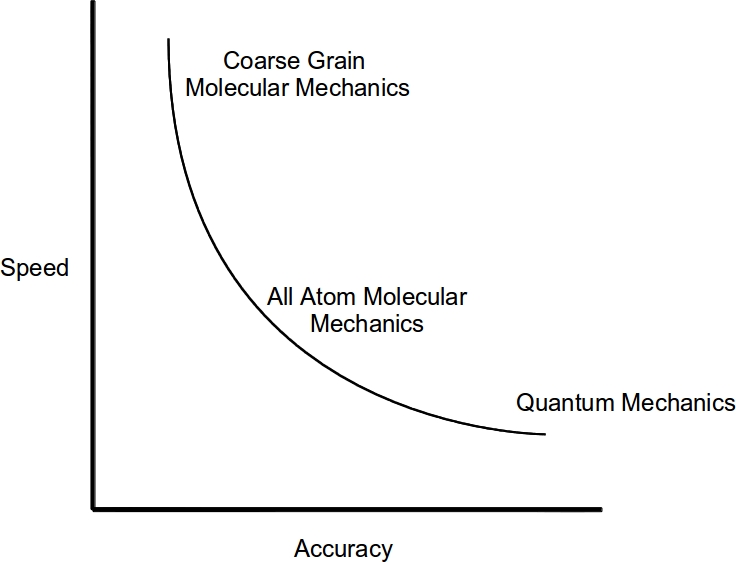
\includegraphics[width=0.7\textwidth]{figures/conservation_of_annoyance.png}
\caption{To an extent it is always possible to either increase accuracy or decrease running time, or the cost of an experiment.
New scientific methods should allow one to increase accuracy while not spending additional time.}
\label{figure:pdb_growth}
\end{center}
\end{figure}

%\begin{figure}[h]
%    \centering
%    \begin{subfigure}[b]{0.3\textwidth}
%        \centering
%        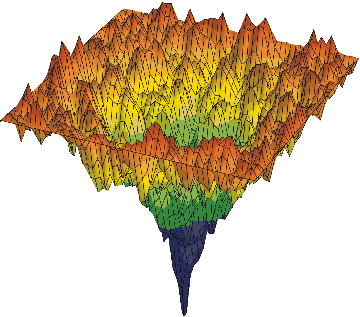
\includegraphics[width=\textwidth]{figures/drysurf.png}
%        \label{fig:dry}
%        \caption{}
%    \end{subfigure}%
%    \begin{subfigure}[b]{0.3\textwidth}
%        \centering
%        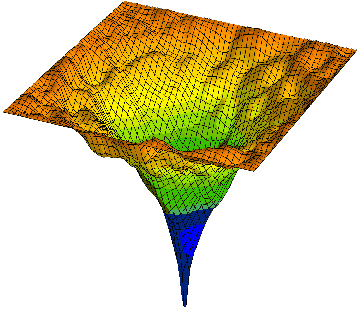
\includegraphics[width=\textwidth]{figures/wetsurf.png}
%        \label{fig:wet}
%        \caption{}
%    \end{subfigure}
%    \caption{The protein energy surface is roughly funnel shaped}
%    \label{fig:funnel}
%\end{figure}

Because of the evolutionary cost of mis-folded proteins, proteins have been selected to minimize mis-folding, making the general shape of the potential energy surface roughly funnel shaped with the native structure at the minimum \cite{leopold1992protein}.
Despite this shape, the energy landscape of proteins is a very ``jagged'' surface with a large number of local minima \cite{tsai1999folding}.

Even the smallest enzyme contains 62 amino acids, and has thousands of degrees of freedom \cite{chen19924}, and larger enzymes are regularly more than 1000 amino acids.
The number of degrees of freedom of these systems make any attempt to analytically solve for a global minimum energy conformation impossible, and require other methods of generating plausible conformations.
In order to compensate for this a number of different sampling methods have been developed.

\subsection{Sampling Methods}
\label{subsection:sampling_methods}

\subsubsection{Cyclic Coordinate Descent}
\label{subsubsection:cyclic_coordinate_descent}

\subsubsection{Analytic Loop Closure}
\label{subsubsection:analytic_loop_closure}

\subsubsection{Monte-Carlo Sampling}
\label{subsubsection:monte_carlo}
Monte-Carlo simulations \cite{li1987monte}.

\subsubsection{Minimization}
\label{subsubsection:minimization}

\subsection{Energy Functions}
\label{subsection:energy_functions}

\begin{equation}
E \left(r^N \right ) = E_\mathrm{bonds} + E_\mathrm{angles} + E_\mathrm{dihedrals} + E_\mathrm{nonbonded}
\label{equation:opls}
\end{equation}

\begin{equation}
E_\mathrm{bonds} = \sum_\mathrm{bonds} K_r (r-r_0)^2
\end{equation}

\begin{equation}
E_\mathrm{angles} = \sum_\mathrm{angles} k_\theta (\theta-\theta_0)^2
\end{equation}

\begin{equation}
E_\mathrm{dihedrals} = \sum_{i=1\dots4} {\frac {V_i} {2} \left [ 1 + \cos \left ( i * (\phi-\phi_0) \right ) \right ] }
\end{equation}

\begin{equation}
\begin{split}
E_\mathrm{nonbonded} = \sum_{i>j} f_{ij} 
                \left (
                        \frac {q_i q_j e^2}{r_{ij}}
                    + 4 \epsilon_{ij} 
                    \left  [  
                        \left ( \frac{\sigma_{ij}}{r_{ij}}\right )^{12}
                      - \left ( \frac{\sigma_{ij}}{r_{ij}}\right )^{6}
                    \right ]
                \right )
\\
f_{ij} = 
  \begin{dcases*}
   0    & if $i$ and $j$ are separated by 2 or fewer bonds\\
   0.5  & if $i$ and $j$ are separated by 3 bonds\\
   1.0  & otherwise
  \end{dcases*}
\end{split}
\end{equation}


Where $\sigma_{ij} = \sqrt{\sigma_{ii} \sigma_{jj}}$ and $\epsilon_{ij} = \sqrt{\epsilon_{ii}\epsilon_{jj}}$ \cite{jorgensen1996development}.
